% !TEX root = ../main.tex

\chapter{绪论}
近些年来,由于互联网的普及,计算机技术的发展和各种社交网络的兴起,视频和图片数据以爆炸性的速度快速增长。如何对海量的图像数据进行处理以及分析促进了一系列的计算机视觉技术的飞速发展,图像检索技术是其中一个核心研究方向。早期基于文本的图像检索极大依赖于标注者的主观判断的标签,检索效率以及性能低下同时需要耗费大量的人力资源,难以应用于海量的互联网图像数据检索。基于内容的的图像检索(Content Based Image Retrieval, CBIR)通过算法自动提取图像的视觉特征来衡量图片之间的相似度,从而实现在数据库中进行图像检索的目的,极大的节省了人工标注耗费的人力、物力和财力。为了提高检索速度以及降低存储开销,哈希编码以及量化编码方法被广泛应用到了图像检索领域,成为解决超大规模图像检索问题的重要解决方案。 本章重点介绍大规模图像检索算法的研究背景以及意义,概要的介绍了图像检索算法发展历史, 详细介绍了基于深度哈希的大规模的图像检索算法。 本章最后介绍了这篇论文的章节安排以及概括介绍每个章节包含的主要内容。
\section{本研究的背景及意义}
在大数据、移动互联网、计算机技术、传感器技术、云计算等前沿技术的发展以及经济社会急速发展的需求下,人工智能(artificial intelligence)作为被视为驱动新一轮产业变革的技术受到了世界各国的广泛关注。 广义的人工智能\cite{russell2010artificial} 包含对大数据的处理分析,自动推理能力,学习能力,以及解决问题的能力。而对以往存储的大数据信息的检索是后续学习与分析的基石,而图像检索便是其中关键的一部分。 \par
基于内容图像检索自从1990年代以来便受到了计算机视觉研究人员广泛的探索~\cite{zhou2017recent}。如图所示, 典型的图像检索一般是指图片中进行特征提取,完成从原始图像空间到特征空间的映射,同时图片的特征应当保留原始图片的语义一致性。语义相似的图片的特征应当尽量接近,相反,语义不同的图片特征应该尽量远离。早期基于人工特征如 (SIFT , GIST, etc ) 的图像检索方法一般面临 ``语义鸿沟'' \cite{li2016socializing} 的难题, 基于人工提取构建的低层次特征难以真实描绘保存高层次的语义特征。2012年, Krizhevsky 等人提出 ALexNet~\cite{krizhevsky2017imagenet} 并且在大规模视觉识别挑战赛中以比第二名低 $10.8\%$ 的 top-5 错误率的性能取得了冠军。自此,基于深度学习进行端对端的特征学习成为了计算机视觉领域的主流。通过设计不同的卷积神经网络(Convolutional Neural Network, CNN)结构,以及采用不同度量学习损失函数,基于深度学习的图像检索方法取得了引人注目的精度提升。自2021年来, Google 首次将自然语言处理领域的基于自注意力机制 (self-attention mechanism)的深度学习模型 transformer 应用到了计算机视觉领域, 并且在多个任务达到最先进水平。由于视觉 Transformer 具有较低的归纳偏置 (inductive bias), 在具有大规模监督数据的领域,它取得了比 CNN 更优异的图像表征学习能力。 因此探究其在图像检索领域的应用,也成为了当前的研究热点之一。  \par
另一方面,在图像领域的实际应用中。由于现在自媒体社交网络、计算机硬件、互联网技术以及数字成像技术的飞速发展,图像数据库的数据量也以爆炸性的速度急剧增长。例如, 据估计社交网络巨头 Facebook 公司用户每日上传的图片数据接近3.5亿,而 Flicker 公司每日的图像数据也达到接近1600万。传统的基于深度学习的检索方法一般采用2048纬度的64位浮点向量, 存储每一张图片需要占用16 千字节 (Kilobyte, KB)。同时, 由于一般使用欧式距离或者余弦距离来刻画图片在特征向量空间的相似度,计算开销大,检索速度慢,无法满足极大规模图像检索对于存储以及检索速度的要求。 基于深度哈希的检索方法由于将图像映射成低维二进制向量,使用汉明距离或者非对称距离计算相似度,是大规模图像检索的理想的解决方案,探究如何提高其性能同时具有较高的学术价值,以及工业应用价值。\par
本文致力于探究大规模的图像检索技术, 提高图像检索的可扩展性,以及检索性能,具有以下方面的重要应用价值:
\begin{enumerate}
    \item 电商搜图: 传统通过文字描述搜索产品有较大的局限性,用户往往很难用文字精确描述想要的产品。 基于视觉图片的图像检索功能可以很好解决这一痛点,目前已经广泛被主流的电商网站,如阿里巴巴、京东等,采用来大幅度提高客户的购物体验。
    \item 智能安防: 基于图像检索的行人重识别技术是智慧城市智能安防的基石。通过对城市大量监控摄像头拍摄的行人照片进行结构化的存储, 行人重识别可以帮助警察迅速大规模筛查可疑犯罪对象,迅速建立防控机制,以最快的速度预防或者制止犯罪行为。 
    \item 遥感检索: 基于视觉的遥感图像检索应用在卫星拍摄储存的遥感大数据库中, 可以帮助监控农业发展和地理位置定位。同时,遥感图像检索还能被应用在灾难解救的场景。 例如,在洪水灾害来临时,遥感检索可以帮助实时获取以及预测洪水水位以及风暴潮,对后续抗灾可以发挥关键作用。
    \item 版权保护: 图像检索还能应用在版权保护领域, 通过对已有版权图像的存储。通过对有争议的图片与数据库版权图像的检索对比, 可以有效确定版权归属。
    \item 医疗诊断: 医疗图像检索可以帮助医生诊断病情。医生可以通过检索相似的过往的医疗病例,对当前的医疗影像数据进行分析与判断,增加诊断的准确度。同时,医疗研究机构可以通过医疗图像检索加强教学实力。教授可以通过检索相关的病例,强化学生对于医疗图像病症的识别分析能力。
\end{enumerate}

\section{国内外发展历史和研究现状}
自从1990年以来, 图像检索作为计算机视觉领域的一个主流任务受到了国内外研究人员的广泛关注。 本章以时间为轴,梳理了一下图像检索的发展已经介绍目前的研究现状。我们首先介绍了早期基于手工设计特征的图像检索方法。由于深度学习的发展, 基于卷积神经网络端对端学习图像特征成为了主流。我们回顾了基于图像检索深度学习的主干网络发展历程。然后, 我们简要的介绍基于深度学习的图像检索主流架构方法。最后,我们详细介绍基于哈希算法的大规模图像检索的背景与发展。
\subsection{基于手工特征的图像检索}
\label{sec:manual}
基于手工特征的图像检索发展也可以简要分成两个阶段。 (1) 基于全局特征提取方法 (2) 基于局部特征提取方法
\subsubsection{基于全局特征提取}

基于全局特征提取算法的算法通常基于纹理特征~\cite{park2002fast,wang2014content}、图片色彩~\cite{wang2011interactive}\cite{wengert2011bag}、 轮廓~\cite{wang2006large}来描述图片的内容,并且生成一个全局的表征向量。GIST~\cite{friedman1979framing,torralba2003context} 是一种典型的全局特征提取算法被广泛应用在检索领域, 由于其不需要对图像进行分割以及进行局部特征提取, 具有计算复杂度低以及运行速度快等优势~\cite{zhou2017recent}。然而, 基于全局特征提取的方法很难保留局部的细粒度特征, 难以取得优异的性能。
\subsubsection{基于局部特征提取}
基于局部特征提取的方法一般包含三个关键的步骤~\cite{zhou2017recent}: ``\textbf{兴趣点检测}''、 ``\textbf{特征描述}''、 ``\textbf{特征融合}''。``\textbf{兴趣点检测}'' 是指通过算法可靠的标注出图像中包含关键内容的角点。在2003年, Google的视频检索系统采用了 MSER~\cite{matas2004robust}检测器取得了仿射不变的特征点检测效果。 之后,Lowe 等人提出了 Hessian-affine 检测器~\cite{lowe2004distinctive}, 可以生成仿射不变(affine-invariant)以及尺度不变 (scale-invaraint)的特征, 以及一定程度上可以对光照条件以及观察点的改变不敏感的特征,随后被广泛应用在检索领域~\cite{philbin2007object}。在2006年, FAST~\cite{rosten2008faster} 通过判断一个像素与周围的连续像素是否处于一个灰度区间判断其是否是一个角点, 具有检测速度快的优点, 但是不具备仿射以及尺度不变性。 在提取完兴趣点后, ``\textbf{特征描述}'' 算法从将兴趣点所在的局部视觉特征提取出特征描述子 (descriptor)。一般的特征描述子应该具有旋转不变性、仿射不变性以及对噪声以及光照改变不敏感~\cite{zhou2017recent}。SIFT ~\cite{lowe2004distinctive}算法是最常被使用的局部特征提取算法。SIFT 通过高斯差分函数 (DoG)识别对尺度以及旋转不变的关键点,通过计算领域像素梯度为每个关键点分配方向角度从而实现旋转不变性。最后再为每个关键点计算光照视角不变的128维的特征描述子。随后, PCA-SIFT~\cite{ke2004pca} 通过降低SIFT生成的特征向量维度来提高匹配的速度。2012年, 另一个基于SIFT的改进算法 RootSIFT~\cite{arandjelovic2012three} 通过对SIFT提取的特征进行L1正则化并且取平凡根, 极大的提高了检索的精度, 成为了基于SIFT特征提取的标准算法。 SURF~\cite{bay2006surf} 是另一种常用的特征提取方法, 在取得与SIFT接近的检索精度的同时,提高了检索的速度。 ``\textbf{特征融合}''将SIFT或者SURF生成的多个局部特征描述子融合生成一个全局特征向量, 便于后续图片检索计算。常用的有特征融合方法有 BoF (Bag of Features, Bag of Visual Words) 、 VLAD (Vector of Local Aggregated Descriptors)和 FV (Fisher vector)三种。
\subsection{基于深度学习的主干网络发展}
近些年来,深度学习发展迅猛。深度学习通过神经网络训练,以端到端的方式进行特征学习,有强大的表征能力,在计算机视觉领域以绝对的性能优势超越传统基于手工设计特征的算法。在图像检索领域,基于深度学习的算法也已经成为了当前的主流。我们以时间为轴, 梳理展示在图像检索领域使用的基础主干神经网络基础架构。
\subsubsection{卷积神经网络}
卷积神经网络(CNN)在1980年代开始被应用于视觉领域的任务。1989年, LeCun 提出了第一个卷积神经网络\cite{lecun1989backpropagation} 用于手写邮编识别。和早期基于全链接的神经网络相比, 卷积神经网络采用局部连接和权值共享,使得网络更加易于优化,同时降低了模型复杂度,减少了模型过拟合的风险。\par
1998年, LeNet~\cite{lecun1998gradient} 是一个具有三个卷积层以及两个全链接层的端到端的神经网络结构, 采用用反向传播算法(Back propagation)~\cite{} 进行梯度下降训练。LeNet在手写数字识别的任务中取得了不错的效果, 被视为当代卷积神经网络的雏形。\par
在大规模的训练数据集的出现, 例如 Pascal 和 ImageNet, 以及计算机硬件算力极速增长的背景下, 2022年, Krizhevsky~\cite{krizhevsky2017imagenet} 提出一个深层的卷积神经网络 AlexNet, 在ImageNet 大规模视觉识别挑战(ILSVRC 2012)中获得冠军。AlexNet 一共包含8层, 由五个卷积层和3个全链接层组成, 包含了6000万的参数量。AlexNet首次采用 ReLU~\cite{glorot2011deep} 激活函数, 证明在深层网络训练中, ReLU 明显优于之前通用的 sigmoid 激活函数, 解决了Sigmoid激活在深层次网络结构中会导致梯度弥散的问题。 同时AlexNet 在训练时采取 Dropout ~\cite{srivastava2014dropout} 策略,以一定概率随机失活一部分神经元降低模型的过拟合。同时,也采用了数据增强的技术增大了模型的泛化能力。AlexNet 首次设计深度神经网络并且成功解决大规模的图像识别任务, 开启了深度学习研究以及应用的大浪潮,成为了计算机视觉任务的主流基本网络架构。 \par
2014年, Simonyan and Zisserman~\cite{simonyan2014very} 提出了 VGG 网络。 VGG 从网络结构深度的角度来提升CNN的性能。通过使用3*3的小尺寸卷积核作为所有卷积层的标准, VGG 包括了最低11层到最高19层 (VGG-11、 VGG-13、 VGG-16、 VGG-19)等变种, 证明了提高模型的深度可以更好的学习图像中的视觉特征。 随后 GoogLeNet~\cite{szegedy2015going} 提出同时学习多尺度的图像特征。通过使用同时使用不同大小的卷积核(5*5、3*3、1*1)对图像进行卷积操作, 以及在通道维度进行拼接, 可以学习不同粒度的图像特征。\par
神经网络设计在网络结构深度方面的探究遇到了瓶颈。经验角度来看, 增加网络的层数可以帮助提取复杂的图像特征, 从而取得更好的结果。然而, 研究人员发现深度学习训练时增加网络层数, 模型训练准确度和测试会在饱和后开始急剧下降, 也就是面临模型退化难题。导致训练失败的主要原因是深层网络训练的梯度消失和梯度爆炸。为了解决这个问题, 2015年, Kaiming He 提出了残差网络 ResNet~\cite{he2016deep}。 ResNet 提出恒等映射 (Identity mapping)和 残差映射 (residual mapping)来解决梯度消失或者弥散的问题, 在 ILSVRC-2015 夺得冠军, 成为了主流计算机视觉领域任务的基本主干模型。\par
2017年的CVPR的最佳论文 DenseNet ~\cite{huang2017densely} 提供另一种解决梯度消失的方案。通过在每个denseNet 块中对每个卷积层生成的特征图进行连接, 加强了特征重用,大幅度降低了模型的参数量, 也缓解了模型退化的问题。 \par
利用深度的卷积神经网络模型, 计算机视觉任务取得了惊人的进步, 在如图像识别领域甚至达到了人类的水平。 然而, 以上基础卷积神经网络模型基于全局图像特征提取, 难以达到人类观察图像时的注意力分配。因此基于注意力的学习机制 (attention mechanism)也被引用至视觉领域模型, 帮助CNN 关注局部重点区域特征,提高视觉信息处理的准确性。常见的注意力机制的算法有: ``通道注意力(channel attention)'', 在通道的维度生成注意力掩码~\cite{hu2018squeeze,liu2022spatial, zhang2018context,gao2019global,yang2020gated, chen2019you}。 ``空间注意力 (spatial attention)'', 在空间域计算声称注意力权重来选择重要的区域特征~\cite{wang2018non,gregor2015draw,mnih2014recurrent, jaderberg2015spatial}。通过引进注意力机制, 深度学习模型对图像特征提取进一步加强, 在图像识别任务的准确度已经超过人类水平。
\begin{figure}[!htp]
    \centering
    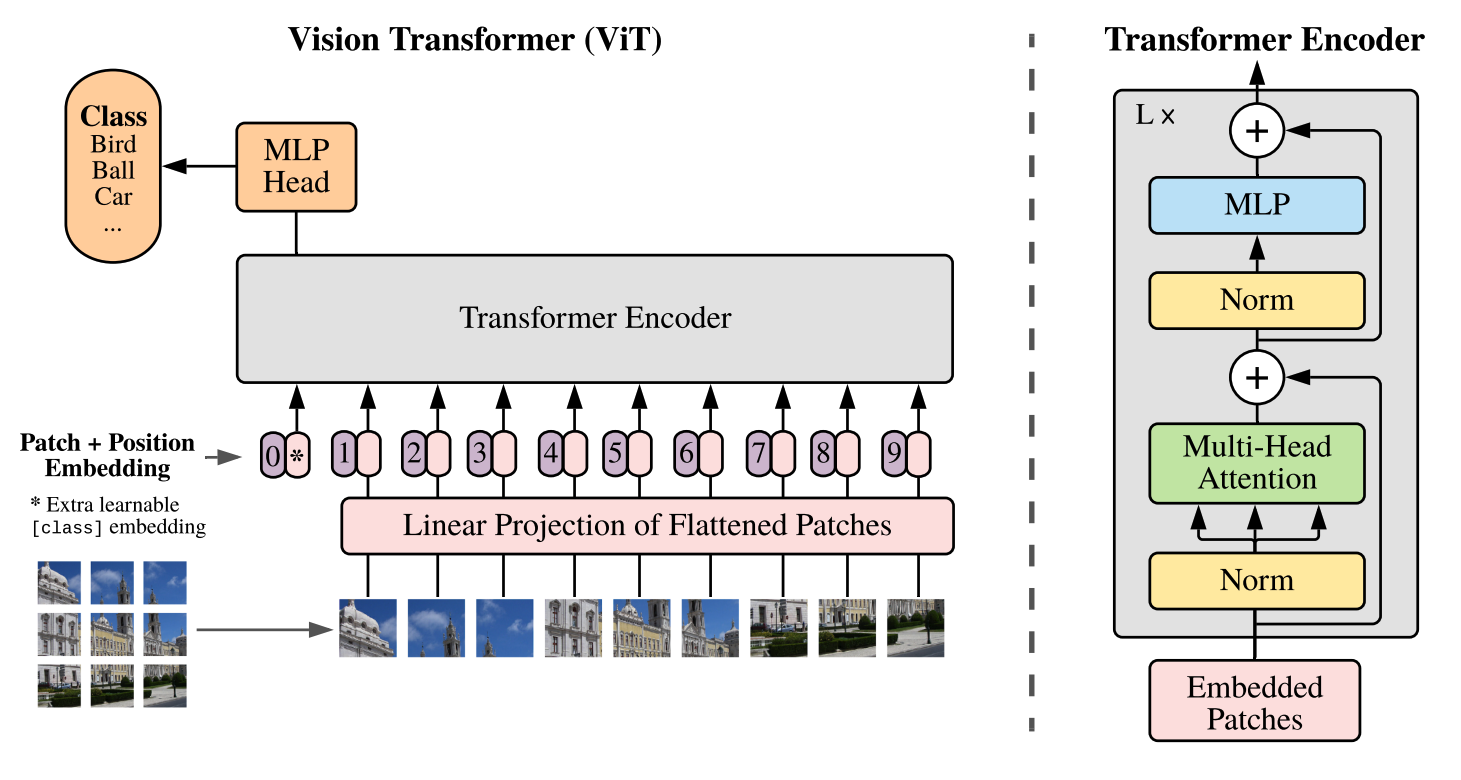
\includegraphics[width=14cm]{vit.png} \\
    \bicaption[视觉转换器的基础框架]
      {视觉转换器的基础架构~\cite{dosovitskiy2020image}}
      {The framework of Vision Transformer}
   \label{fig:vit}
  \end{figure}


\subsubsection{视觉转换器}
在2020年底, 完全基于自注意力机制 (self-attention)的视觉转换器 (vision transformer)的横空出世挑战了传统CNN在计算机视觉领域的绝对优势地位, 并在多个视觉任务超过ResNet等CNN模型的性能。Transformer~\cite{vaswani2017attention}最初由Google在2017年提出, 应用在自然语言处理领域(Natural Language Processing, NLP)代替传统循环神经网络(RNN)进行序列建模。这种完全基于自注意力机制的深度模型相比较于RNN的模型具有可并行化计算以及低内存开销的优势, 并且在一系列的机器翻译任务中取得优异的性能。Devlin 等人将 Transformer \cite{devlin2018bert} 应用至无监督NLP模型预训练任务, 并在当时11个任务上取得最先进的结果。随后, OpenAI开发了GPT-3~\cite{brown2020language}, 一个具有1750亿参数的大模型, 并且在45 TB的数据进行预训练。模型在多个NLP的任务都取得了极佳的性能, 包括机器翻译 (machine translation) 、 视觉问答(visual question answering)等。基于Transformer的模型展示了强大的表征能力,并且成为了NLP领域的主流模型。\par

2020年, Google的研究人员首次将基于序列建模的NLP基础模型Transformer扩展到计算机视觉任务, 设计了 Vision Transformer~\cite{dosovitskiy2020image} 。如Fig.~\ref{fig:vit}所示, Vision transformer 包含标准的 Transformer 编码器。
\begin{figure}[!htp]
    \centering
    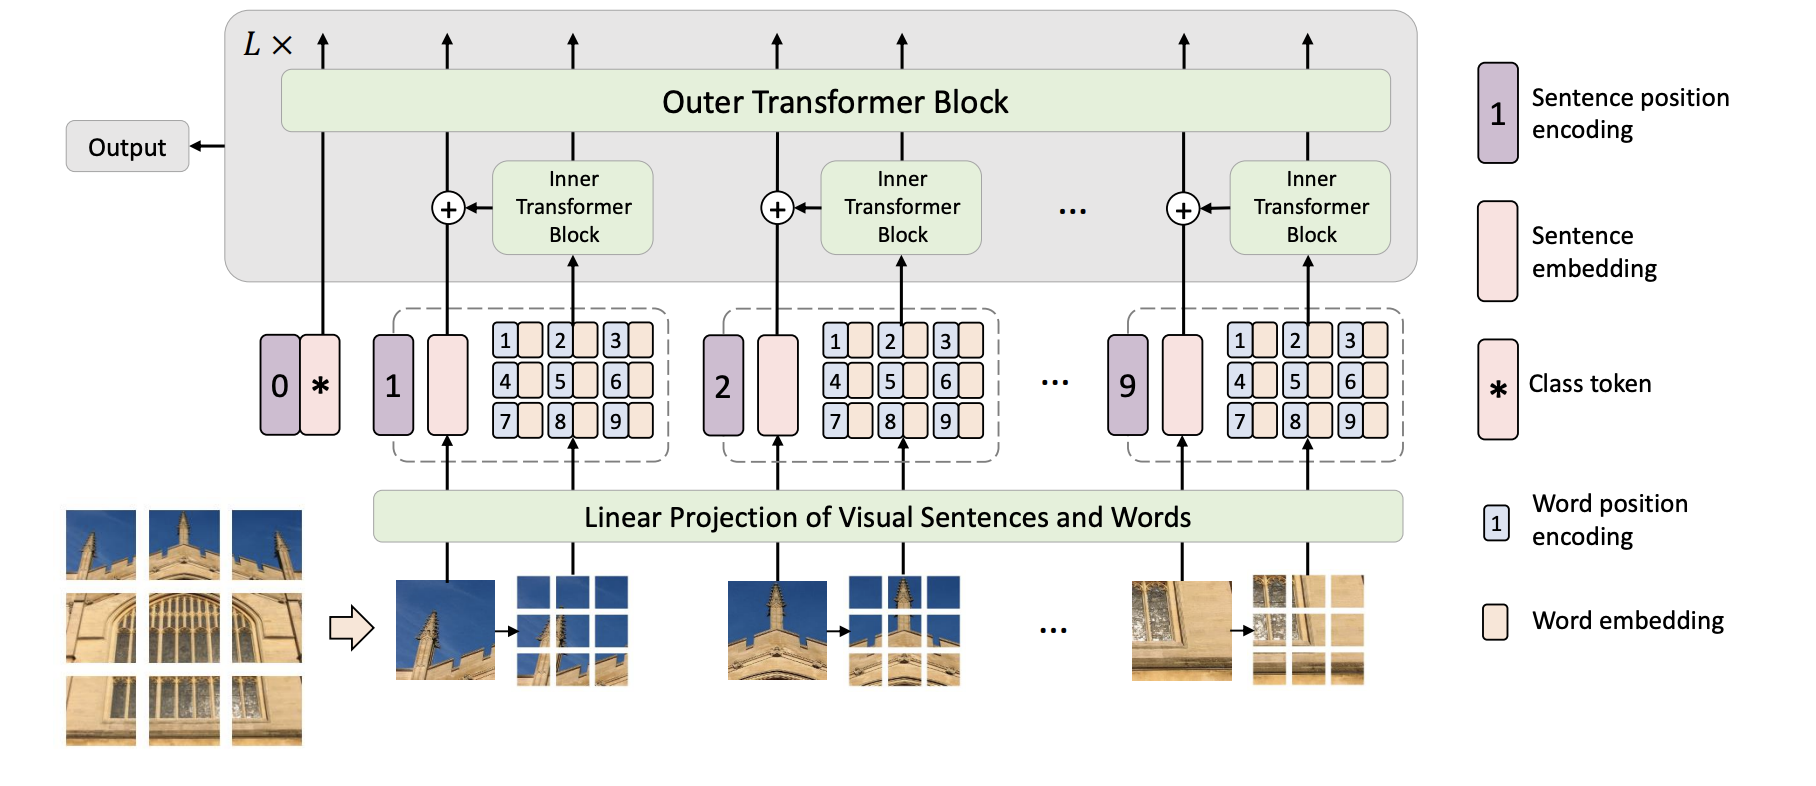
\includegraphics[width=15cm]{tit.png} \\
    \bicaption[视觉转换器变种的基础框架, 图~\cite{han2021transformer}]
      {Transformer in Transformer 的基础架构~\cite{han2021transformer}}
      {The framework of  Transformer in Transformer}
   \label{fig:tit}
  \end{figure}

其主要模块是基于多头的注意力机制 (Multi-head Attention, MHA):
\begin{equation}
    \text { MultiHead }(Q, K, V)=\text {Concat}\left(\text {head}_1, \ldots, \text {head}_{\mathrm{h}}\right) W^O,
\end{equation}
\begin{equation}
    \text {head}_{\mathrm{i}}=\operatorname{Attention}\left(Q W_i^Q, K W_i^K, V W_i^V\right).
\end{equation}
其中 Query向量 ($Q$), Key向量 ($K$), Value向量 ($V$) 是对应序列中每一个token的三个不同的矩阵, h 是代表并行的自注意力数量, $W_i^Q$, $W_i^K$, $W_i^V$ 是对应的每一个自注意力的投射矩阵, MHA通过将多个自注意力得到的表征结果进行融合, 实现模型关注序列不同的token的效果。同时, 自注意力的表述如下:

\begin{equation}
    \operatorname{Attention}(Q, K, V)=\operatorname{softmax}\left(\frac{Q K^T}{\sqrt{d_k}}\right) V.
    \label{eq:attention}
\end{equation}
其中 $d_k$ 是 Key向量的维度。\par
为了使Transformer能处理2D的图像数据, 如\ref{fig:vit}所示, 将图片$\mathbf{x} \in \mathbb{R}^{H \times W \times C}$ 切割成一系列的图片块$\mathbf{x}_p \in \mathbb{R}^{N \times\left(P^2 \cdot C\right)}$。 其中 $H$, $W$, $C$ 是图片的高、宽、以及通道数。$N=H W / P^2$ 是得到的图片块的数量。通过对图片块进行投影降维, 可以得到类似于在自然语言处理领域的序列输入:
\begin{equation}
    \mathbf{z}_0=\left[\mathbf{x}_{\text {class }} ; \mathbf{x}_p^1 \mathbf{E} ; \mathbf{x}_p^2 \mathbf{E} ; \cdots ; \mathbf{x}_p^N \mathbf{E}\right]+\mathbf{E}_{p o s}
\end{equation}
其中 $E$是投影矩阵, 将图像块降维成低维向量, $E_{pos}$ 是图片块的位置嵌入(Position embeddings)。由于Vision Transformer 比CNN具有更少的归纳偏置 (inductive bias),
\begin{figure}[!htp]
    \centering
    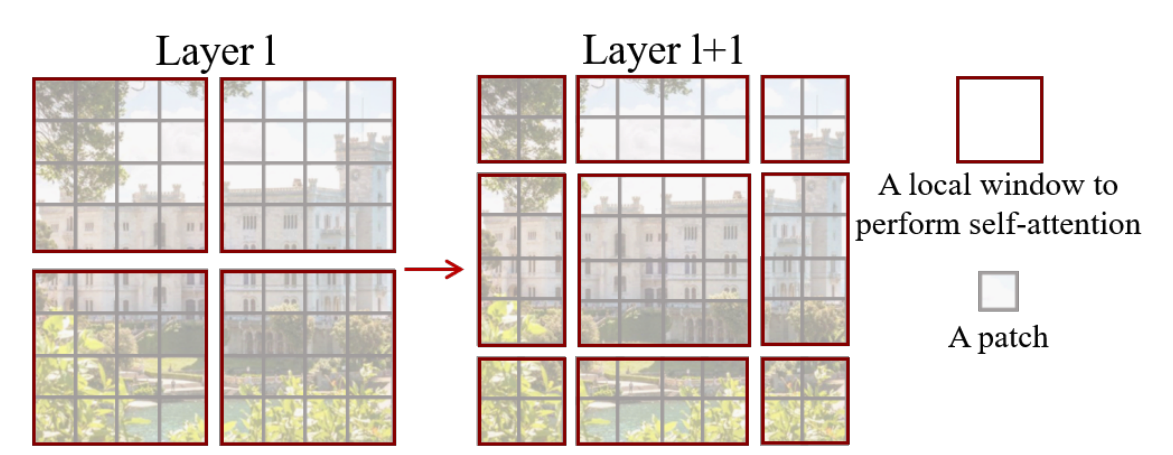
\includegraphics[width=15cm]{swin.png} \\
    \bicaption[移动窗口自注意力的计算机制, 图~\cite{liu2021swin}]
      {移动窗口自注意力的计算机制~\cite{liu2021swin}}
      {The Illustration of Shifted Window Multi-head Self Attention }
   \label{fig:swin}
\end{figure}

在小规模数据集上预训练时, 没有达到CNN的性能, 然而在大规模数据集 (JFT-300M)上训练, Vision transformer 取得更优的图像分类效果。 随后, Vision transformer 开始被应用在多个计算机视觉任务, 如目标检测(Object detection) ~\cite{carion2020end, zhu2021deformable}、语义分割 (semantic segmentation)~\cite{zheng2021rethinking, xie2021segformer, strudel2021segmenter, jin2021trseg, zhu2021unified}、 图像处理 (image processing)~\cite{chen2021pre} 等领域。 随后 Touvron等人基于原始Vision transformer提出Deit, 仅在ImageNet上进行训练, 取得 $83.1\%$的分类准确度。 在使用CNN 进行知识蒸馏 (knowledge distillation)后, 取得最高达 $85.2\%$的准确度。\par

2021年, 传统的vision transformer只能刻画图片块之间的联系, 而忽略了一个图片块内部的特征。 为了解决这个问题, 如图\ref{fig:tit}, Han 等人提出一个transformer in transformer的架构, 对原始图片块继续细分成更小的图片块, 并且同时对粗粒度和细粒度的图片块进行建模。随后, CAT~\cite{lin2022cat} 和 Twins~\cite{chu2021twins} 提出交替在层间使用全局以及局部的注意力机制来减少计算复杂度以及提高表征能力。\par

由于如Eq.~\ref{eq:attention}所示, 自注意力力机制的计算复杂度随着图片块数量$N$的增长成平方增长, 使得基础的vision transformer模型无法应用在高分辨率的视觉任务中。 2021年, ICCV的最佳论文奖得主 Swin Transformer~\cite{liu2021swin}提出在移动窗口内进行自注意力计算 (shifted-window self-attention), 如Fig.~\ref{fig:swin}所示, 图左是在第l层的窗口划分, 其中自注意力的计算局限于红色的窗口内。假设每一个窗口包含$M \times M$个图片块, 那么基于窗口的自注意力机制的计算复杂度 (W-MSA)可以由以下的公式表示:
\begin{equation}
    \Omega(\text { W-MSA })=4 h w C^2+2 M^2 hwC.
\end{equation}

其中$hw$是图片块的数量。由此可知, Swin-transformer 的计算复杂度随着图像大小可以呈线性增长, 具有可扩展性。Swin Transformer在图像分类, 目标检测等领域都达到了最先进的性能, 开始成为计算机视觉领域的主干模型~\cite{liu2021swinnet,liu2022video, huang2022swin, cao2021swin, ma2022swinfusion}。在本文中, 我们第一个探索vision transformer在大规模图像检索领域的应用,并且取得了优异的性能。
\subsection{基于深度特征的图像检索}
在深度学习时代的图像检索方法主要分为两种: (1) 基于预训练CNN的特征提取 (2)基于任务的微调。早期的基于深度学习的检索方法基于两阶段检索, 即使使用用在图像分类数据集如ImageNet进行分类任务训练后的CNN代替基于人工的特征提取方法,如SIFT, 进行特征提取, 第二阶段如Sec.~\ref{sec:manual}, 使用 VLAD、 BoW 或者 FV 生成全局的表征向量。 而基于端到端的检索, 使用图像的监督标签, 端到端训练生成用于图像检索的表征向量, CNN 会在监督训练的过程中调整学习适用于特定任务的图像特征。 
\subsubsection{基于预训练CNN的特征提取}
一部分基于预训练CNN提取的特征工作一般也包含两个阶段: ``特征提取'' 与 ``特征聚合''。``特征提取'': 如图所示, 一部分工作从全连接层得到特征向量, 类似手工特征提取方案的全局特征描述符, 然后使用PCA 降以及标准化~\cite{sharif2014cnn,gong2014multi}。然而, 基于全连接层的特征向量损失了图像的空间信息, 缺乏局部几何不变性~\cite{gong2014multi}。因此, 另一部分研究人员研究使用卷积层后的特征图进行图像检索。2016年, Razavian~\cite{razavian2016visual} 提取CNN最后一个卷积层的多尺度特征, 并且通过空间池化(spatial pooling) 降维用于检索。随后 Morere 提出嵌套不变池化 (nested invariance pooling )来生成用于检索的全局描述符。
\subsubsection(基于任务的微调)

\subsection{基于深度哈希的大规模检索}


\section{本文章节安排与研究内容}